\documentclass{amsart}

\include{RDTP-Preamble}

\begin{document}

\title{The balanced tensor product of module categories}

\begin{abstract}
The balanced tensor product $M \otimes_A N$ of two modules over an algebra $A$ is the vector space corepresenting $A$-balanced bilinear maps out of the product $M \times N$.  The balanced tensor product $\cM \boxtimes_{\cC} \cN$ of two module categories over a monoidal linear category $\cC$ is the linear category corepresenting $\cC$-balanced right-exact bilinear functors out of the product category $\cM \times \cN$.  We prove that the balanced tensor product exists, provided the monoidal linear category is finite and rigid, and the module categories are finite.
\end{abstract}




%A key role in the theory of tensor categories is played by the balanced tensor product $\cM \boxtimes_\cC \cN$ which is a higher dimensional analogue of the tensor product of a right and a left module over a non-commutative ring.  The balanced tensor product is characterized by a universal property, but such a characterization does not guarantee existence.  In this paper, we give a construction of the balanced tensor product for finite tensor categories (in the sense of Etingof-Ostrik) and their finite module categories.  This generalizes results of Etingof-Nikshych-Ostrik in the semisimple case.  Explicitly, we realize the balanced tensor product over $\cC$ as a category of bimodule objects in $\cC$.

\author{Christopher L. Douglas}
\address{Mathematical Institute\\ University of Oxford\\ Oxford OX1 3LB\\ United Kingdom}
\email{cdouglas@maths.ox.ac.uk}
\urladdr{http://people.maths.ox.ac.uk/cdouglas}
      	
\author{Christopher Schommer-Pries}
\address{Department of Mathematics\\ Max Planck Institute for Mathematics \\ 53111 Bonn \\ Germany}
\email{schommerpries.chris.math@gmail.com}
\urladdr{http://sites.google.com/site/chrisschommerpriesmath}

\author{Noah Snyder}
\address{Department of Mathematics\\ Indiana University\\ Bloomington, IN 47401\\ USA}
\email{nsnyder@math.columbia.edu}
\urladdr{http://www.math.columbia.edu/\!\raisebox{-1mm}{~}nsnyder/}

\thanks{CD was partially supported by a Miller Research Fellowship and by EPSRC grant EP/K015478/1, CSP was partially supported by NSF fellowship DMS-0902808 and the Max Planck Institute for Mathematics, and NS was partially supported by NSF fellowship DMS-0902981 and DARPA HR0011-11-1-0001.
}


\maketitle	

\tikzexternaldisable

%\setcounter{tocdepth}{2}
%\tableofcontents

Needless to say, the tensor product $V \otimes W$ of vector spaces is a fundamental algebraic operation, as is the balanced tensor product $M \otimes_A N$ of two modules over an algebra.  There are categorical analogs of the notions of vector space, algebra, and module, namely (abelian) linear category, monoidal linear category, and module category.  Deligne~\cite{MR1106898} constructed a categorical tensor product $\cK \boxtimes \cL$ of finite linear categories.  Etingof, Nikshych, and Ostrik~\cite{0909.3140} established the existence of a balanced tensor product $\cM \boxtimes_{\cC} \cN$ of finite semisimple module categories over a finite, rigid, semisimple monoidal linear category over a field of characteristic zero.  We prove that the balanced tensor product exists more generally for not-necessarily-semisimple monoidal linear categories and module categories, over any base field.

The balanced tensor product $M \otimes_A N$ is, by definition, the vector space corepresenting $A$-balanced bilinear maps out of $M \times N$---a map $M \times N \ra L$ is $A$-balanced if precomposing with the action of $A$ on $M$ or on $N$ produces the same map $M \times A \times N \ra L$.  If the balanced tensor product exists, it is certainly unique (up to unique isomorphism); existence is typically established by explicit construction as a quotient of a free abelian group on the product $M \times N$.  Similarly, the balanced tensor product $\cM \boxtimes_{\cC} \cN$ of module categories over a monoidal linear category is the linear category corepresenting $\cC$-balanced right-exact bilinear functors out of $\cM \times \cN$.  Again if the balanced tensor product exists, it is unique (up to an equivalence that is unique up to unique natural isomorphism).  

The only task is to provide an explicit construction of the balanced tensor product that satisfies the corepresentation property.  A crucial tool for the construction is the result, proved by Etingof--Gelaki--Nikshych--Ostrik \cite[Thm 2.11.6]{EGNO}, based on earlier work of Etingof--Ostrik \cite[\S 3.2]{EO-ftc} along the lines pioneered by Ostrik \cite[Thm 1]{MR1976459}, that any finite left module category ${}_{\cC} \cN$ over a finite tensor category $\cC$ is equivalent to the category of right module objects $\Mod{}{B}(\cC)$ in $\cC$, for some algebra object $B \in \cC$; similarly any right module category $\cM_{\cC}$ is equivalent to a category of left module objects $\Mod{A}{}(\cC)$.  It therefore suffices to construct a balanced tensor product of module categories that are presented as categories of module objects, $\Mod{A}{}(\cC)$ and $\Mod{}{B}(\cC)$, and in that case, the category $\Mod{A}{B}(\cC)$ of $A$--$B$-bimodule objects in $\cC$ provides an explicit realization of the product.

\begin{theorem*}
Let $\cC$ be a finite, rigid, monoidal linear category, and let $\cM$ be a finite right $\cC$-module category and $\cN$ a finite left $\cC$-module category.  There exists a finite linear category $\cM \boxtimes_\cC \cN$ corepresentating $\cC$-balanced right-exact bilinear functors out of $\cM \times \cN$.
\end{theorem*}

In Section~\ref{sec:tc-lincat}, we give an expositional overview of linear categories and monoidal linear categories.  In particular, we give a proof of the well known fact that all finite linear categories are equivalent to categories of modules over a finite-dimensional algebra, and a proof of the fact that all right (respectively left) exact linear functors between finite linear categories admit right (respectively left) adjoints.  In Section~\ref{sec:tc-bimod}, we provide a review of aspects of Etingof--Gelaki--Nikshych--Ostrik's theory of module categories, including proofs that all module functors are strong and that adjunctions lift to module adjunctions, and we give a proof, of the fact that module categories are categories of module objects, that isolates and mitigates the rigidity assumption.  In Section~\ref{sec:tc-deligne}, we use the presentation of module categories as categories of modules to prove that the balanced tensor product of module categories exists, and we establish the basic exactness properties of the balanced tensor product.










\CD{Discuss how/where/for what to add back in the refs Mug03, ENO10, JL09, GS12a, GS12b, DNO13, FSV13 // DSPSa, DSPSb // Gre10, Gre11.  Also Tambara!}













%Tensor categories are a higher dimensional analogue of algebras.  Just as modules and bimodules play a key role in the theory of algebras, the analogous notions of module categories and bimodule categories play a key role in the study of tensor categories (as pioneered by Ostrik \cite{MR1976459}).  One of the key constructions in the theory of modules and bimodules is the relative tensor product $M \otimes_A N$ which is universal for $A$-balanced bilinear functions out of $M \times N$.   A similar role is played by the balanced tensor product of module categories $\cM \boxtimes_\cC \cN$ in the theory of tensor categories (for example, see \cite{MR1966524, 0909.3140, MR2511638, MR2909758, 1202.4396, MR3022755, MR3063919}).  This balanced tensor product is often called the relative Deligne tensor product, and it is universal for certain balanced functors.  Since it is defined by a universal property, if it exists this tensor product is unique up to unique isomorphism.  However, in order to prove existence one needs a direct construction.  Such a construction depends on $\cM$, $\cC$, and $\cN$ satisfying certain niceness properties.  

%The balanced tensor product was first constructed by Etingof-Nikshych-Ostrik under the assumption that $\cC$ is a fusion category and $\cM$ and $\cN$ are finite semisimple module categories \cite{0909.3140}.  A construction of the balanced tensor product for certain non-semisimple categories can also be extracted from \cite[Thm 3.1]{1102.3411}.   In this paper, we give a construction of the balanced tensor product under the assumption that $\cC$ is a finite tensor category in the sense of \cite{EO-ftc} and $\cM$ and $\cN$ are finite module categories.  

%\begin{maintheorem}
%If $\cC$ is a finite tensor category, $\cM$ is a finite right $\cC$-module category, and $\cN$ is a finite left $\cC$-module category, then there exists a finite tensor category $\cM \boxtimes_\cC \cN$ representing $\cC$ balanced right exact bilinear functors out of $\cM \times \cN$.
%\end{maintheorem}

%The key result underlying our construction shows that any module category can be realized as a category of modules.  It is due to Ostrik in the fusion case, Etingof-Ostrik for exact module categories, and in the general case appears in Etingof-Gelaki-Nikshych-Ostrik's lecture notes.

%\begin{maintheorem}{\cite[Thm 2.11.6]{EGNO}, \cite[\S 3.2]{EO-ftc}, \cite[Thm 1]{MR1976459}} %\label{thm:EGNO2.11.6}
%	If $\cM$ is a finite left module category over a finite tensor category $\cC$, then there exists an algebra object $A \in \cC$ together with an equivalence of left $\cC$-module categories between $\cM$ and the category of right $A$-module objects in $\cC$.  Similarly, any finite right module category over a finite tensor category is equivalent to a category of left $A$-modules for some algebra object $A \in \cC$.
%\end{maintheorem}

%Using this theorem we have the following explicit construction of the balanced tensor product.

%\begin{maintheorem}
%If $\cC$ is a finite tensor category and $A, B \in \cC$ are algebra objects, then the category of $A\text{-Mod-}B$ objects in $\cC$ together with the obvious forgetful functors satisfies the universal property of the balanced tensor product $(A\text{-Mod}) \boxtimes_\cC (\text{Mod-}B)$.
%\end{maintheorem}

%The balanced tensor product will play a key role in our study of the $3$-category of finite tensor categories and the associated local toplogical field theories in our papers \cite{3TC, DTCI}.  One of our goals in writing this paper is that it can serve as a self-contained introduction to the parts of EGNO's theory which are needed in those papers.  In order to keep this paper self-contained, and to clarify several details of where the assumptions of finiteness and rigidity come into the argument, we have reproved a few results from Etingof, Gelaki, Nikshych, and Ostrik's work and given the proofs of a few results that they left as exercises to the reader.  There is also some overlap with the papers of Greenough \cite{MR2678824, 1102.3411} who restricts his attention to the case of exact module categories.  Another goal is to clarify exactly which assumptions are essential.  In particular in \cite{3TC, DTCI} we do not assume that the base field is algebraically closed.  Furthermore, in the long run we would like to consider the dualizability of non-rigid monoidal categories, so we identify exactly where rigidity appears.
%  \NS{Added the last three sentences.}


\section{Linear categories and tensor categories} \label{sec:tc-lincat}

\subsection{Finite linear categories}

	Let $k$ be a fixed ground field, let $\overline{\Vect}_k$ be the category of (possibly infinite-dimensional) $k$-vector spaces, and let $\Vect_k$ be the category of finite-dimensional $k$-vector spaces.   A {\em linear category} is an abelian category with a compatible enrichment over $\overline{\Vect}_k$. 
A {\em linear functor} is an additive functor, that is also a functor of $\overline{\Vect}_k$-enriched categories. 

\begin{warning}
	In \cite{3TC, DTCI} we will use the phrase ``linear functor" to mean what we call ``right exact linear functor" in this paper.  In the $3$-category of finite tensor categories the $2$-morphisms are assumed to be right exact, because the balanced tensor product of linear categories is only functorial with respect to right exact functors.  Since this paper concerns the definition of the balanced tensor product itself, we will not use the abbreviated convention here.
\end{warning}

Recall the following standard terminology:
\begin{itemize}
	\item[-] An object of a linear category is {\em simple} if it admits no non-trivial subobjects. The endormorphism ring of any simple object is a division algebra over $k$. 
	\item[-] An object $X$ of a linear category has {\em finite length} if every strictly decreasing chain of subobjects $X = X_0 \supsetneq X_1 \supsetneq X_2 \supsetneq  \cdots$ has finite length. 
	\item[-] A linear category is {\em semisimple} if every object splits as a direct sum of simple objects. If in addition every object has finite length, then every object splits as a finite direct sum of simple objects.
	\item[-] A linear category {\em has enough projectives} if for every object $X$, there is a projective object $P$ with a surjection $P \twoheadrightarrow X$. 
\end{itemize}


\begin{definition} % This is from EGNO Definition 1.18.2.
	A linear category $\cC$ is {\em finite} if 
	\begin{enumerate}
		\item[1.] $\cC$ has finite-dimensional spaces of morphisms;
		\item[2.] every object of $\cC$ has finite length;
		\item[3.] $\cC$ has enough projectives%, i.e. every simple object of $\cC$ has a projective cover
		; and
		\item[4.] there are finitely many isomorphism classes of simple objects.  
	\end{enumerate}
\end{definition}

The following proposition is well-known (see for instance \cite[\S9.6]{MR2808160}), and justifies the above definition of finite.

\begin{proposition}
A linear category is finite if and only if it is equivalent to the category $\Mod{A}{}$ of finite-dimensional modules over a finite-dimensional $k$-algebra $A$.
\end{proposition}
\begin{proof}  \NS{Should this be more parallel with the proof of Prop 2.23?}
	Let $A$ be a finite-dimensional $k$-algebra and consider the linear category $\Mod{A}{}$ of finite-dimensional left $A$-modules. The first two conditions for the finiteness of $\Mod{A}{}$ are clearly satisfied, as they are inherited from the corresponding properties of the category of finite-dimensional vector spaces. Because free $A$-modules are projective and every $A$-module $M$ admits the surjection ${}_A A \otimes M \to M$, there are enough projectives. 
	
	Let $M$ be an $A$-module. Every non-zero element of $M$ gives rise to a non-zero map of $A$-modules $A \to M$. If $M$ is simple, the cokernel is necessarily zero.  Thus every simple $A$-module is a quotient of $A$. In particular every simple module occurs as a factor in a composition series for $A$. Since every (finite-dimensional) $A$-module is finite length, there are only finitely many simple modules that occur in any composition series for $A$.  By the Jordan-H\"older theorem there are finitely many simple modules up to isomorphism. Hence the linear category $\Mod{A}{}$ is finite.
	
	Now assume that $\cC$ is a finite linear category. Let $\{X_i\}$ be a set of representatives for the isomorphism classes of simples. Let $P_i \to X_i$ be a surjection, with $P_i$ projective, let $P = \oplus P_i$, and let $A = \Hom_{\cC}(P,P)$. As the morphism spaces of $\cC$ are finite-dimensional, $A$ is a finite-dimensional algebra.  (Note that here the algebra structure on $A$ is defined by $a \cdot b := b \circ a$.)
	
We have an adjunction, which we will show is an equivalence:
	\begin{equation*}
		P \otimes_A (-):\Mod{A}{} \leftrightarrows \cC: \Hom_{\cC}(P,-).
	\end{equation*}
	The left adjoint is given by $P \otimes_A M := \coeq\{ P \otimes A \otimes M \rightrightarrows P \otimes M\}$.  In order to show that this adjunction is an equivalence we need only show that the unit and counit maps are isomorphisms.
Because $P$ is a finite length projective module (and hence a summand of a finite rank free module)\NS{Rewrote this}, we have an isomorphism
\begin{equation*}
	\Hom_{\cC}(P, P \otimes_A M) \cong \Hom_{\cC}(P, P) \otimes_A M \cong M.
\end{equation*}
The composition of the unit map $M \rightarrow\Hom_{\cC}(P, P \otimes_A M)$ with this isomorphism is the identity, hence the unit map is an isomorphism. It only remains to show that the counit 
\begin{equation*}
	ev:P \otimes_A \Hom_{\cC}(P, X) \to X
\end{equation*}
is an isomorphism for every $X$. The counit becomes an isomorphism after applying $\Hom_{\cC}(P,-)$, and so the desired result would follow if we knew $\Hom_{\cC}(P,-)$ reflects isomorphisms. \NS{Changed equivalence to isomorphism several times.}

As $P$ is projective, the functor $\Hom_{\cC}(P,-)$ is exact, and so the fact that it reflects isomorphisms is equivalent to that statement that for all $X$, 
\begin{equation*}
	\Hom_{\cC}(P,X) \cong 0 \quad \textrm{ if and only if } \quad X \cong 0.
\end{equation*} 
By construction this holds for all objects $X$ of length at most 1. We prove that it holds for all objects by induction on the length. 

Suppose that $X$ is an object of $\cC$ and, by induction, that for all objects $Y$ with length strictly less than the length of $X$, we know $\Hom_{\cC}(P,Y) \cong 0$ if and only if $Y \cong 0$. By assumption there exists an exact sequence in $\cC$
\begin{equation*}
	0 \to X' \to X \to X'' \to 0
\end{equation*}
with $X''$ simple, and with the length of $X'$ strictly less than the length of $X$. We obtain an exact sequence:
\begin{equation*}
	0 \to \Hom_{\cC}(P,X') \to \Hom_{\cC}(P,X) \to \Hom_{\cC}(P,X'') \to 0.
\end{equation*}
If the middle term is zero, then all terms vanish. By our induction hypothesis, we conclude that $X'' \cong X' \cong 0$, and hence $X$ itself was zero. Thus $\Hom_{\cC}(P,-)$ reflects isomorphisms, as required.
\end{proof}

\subsection{Adjoints and representability of linear functors}

A property of finite linear categories is that they satisfy the following analog of the adjoint functor theorem.  Although this result is well-known, we were unable to find a proof in the literature.  

\begin{proposition} \label{prop:AFT}
	Let $\cC$ and $\cD$ be finite linear categories and let $G: \cC \rightarrow \cD$  be an additive $\Vect_k$-enriched functor (not necessarily right exact). Then the following conditions are equivalent: 
	\begin{enumerate}
		\item $G$ is left exact;  
		\item $G$ is left exact and satisfies the following {\em solution-set condition:} \\  For each $d \in \cD$ there is a finite set $I$ and a collection of arrows $f_i:d \to G(c_i)$ such that every arrow $h:d \to G(c)$ can be written as a composite $h = G(t) \circ f_i$ for some index $i \in I$ and some $t: c_i \to c$; 
		\item $G$ admits an additive, ${\Vect_k}$-enriched, right exact left adjoint.
	\end{enumerate}
\end{proposition}
\begin{proof} This is a variation of the proof (in the non-linear setting) given in \cite[V.6.Thm 2]{MR0354798} (see also \cite[Ex. 3-M]{MR0166240}).

($3 \Rightarrow 1$) Suppose that $G$ admits a left adjoint $F$. Then $G$ is itself a right adjoint and hence commutes with all limits. In particular $G$ is a left exact functor. 

($2 \Rightarrow 3$) Note that any left adjoint $F$ to $G$ commutes with coproducts, so is an additive functor.  The adjoint $F$ commutes with colimits and so is also right exact.  Finally the left adjoint $F$ is ${\Vect_k}$-enriched if the natural isomorphism of abelian groups $\hom( F(x), y) \cong \hom(x, G(y))$ is compatible with the scalar multiplication by $k$. That follows by naturality and the fact that $G$ is ${\Vect_k}$-enriched.


To construct a left adjoint for $G$, it suffices (and is necessary) to construct for each $d \in \cD$ a universal arrow $d \to G(c)$, that is an initial object of the comma category $(d \downarrow G)$; the left adjoint may then be constructed pointwise as $F(d) = c$. To this end, fix $d \in \cD$ and suppose that $G$ satisfies the solution-set condition. Define the element $w$ of the comma category as the product of the elements $d \to G(c_i)$. Since $G$ is left exact, it commutes with finite limits, and hence the forgetful functor $(d \downarrow G) \to \cC$ creates finite limits. In particular the comma category has all finite limits.  Thus the product of the elements $d \rightarrow G(c_i)$ exists and is given explicitly by
\begin{equation*}
	w := \bigoplus_i f_i :  d \to G( \oplus_i c_i) = \bigoplus_i G(c_i).
\end{equation*}
The morphism spaces of $(d \downarrow G)$ are finite-dimensional vector spaces, and so we may choose a finite basis for $\Hom(w,w)$. Let $v$ be defined as the equalizer of this finite collection of maps together with the zero map. Again, this finite limit exists and may be created in $\cC$. Note that $v$ consequently equalizes the zero map and any linear combination of the basis maps. Thus $v$ equalizes {\em all} endomorphisms of $w$, and hence $v$ is initial; see  \cite[V.6.Thm 1]{MR0354798}. \CD{By construction? Explain this last sentence more?} \CSP{added this and made correction (added zero map)}

($1 \Rightarrow 2$) Finally, suppose that $G$ is left exact. Fix an object $d \in \cD$ and define a class $S_d$ of objects of $(d \downarrow G)$ as follows. An object $(c, f:d \to G c)$ belongs to $S_d$ if and only if for any sub-object $c' \subseteq c$ and factorization $d \to G c' \to G c$ it follows that either $c' \cong 0$ or the inclusion is an isomorphism $c' \cong c$. \CD{Really need given inclusion $c' \subset c$ to be iso, right?} \CSP{yes, changed it.} The class $S_d$ consists of, in the language of \cite[Ex. 3-J]{MR0166240}, those objects $(c,f)$ that are {\em generated} by $d$. If there is a finite set $I$ of isomorphism classes of objects of $S_d$ then a choice of representatives $\{(c_i, f_i)\}_{i \in I}$ forms a collection satisfying the solution-set condition.  \CD{(Should we say more here? As is, no mention of left exact or finite length.)} \CSP{I don't think we really need to say more here. finite length is used in the next paragraph. left exactness of G is not used. The proof here shows that the solution set condition is always satisfied. What that means is that the Kan extension always exists. If G is left exact, then this Kan extension is the right adjoint, as shown earlier. We could add this to the remark after the proof though?}

We must show that the class $S_d$ has finitely many isomorphism classes of objects. Let $q \in \cC$ denote the direct sum of representatives of the isomorphism classes of simple objects in $\cC$. Choose a basis $\{e_j\}$ for the vector space $\hom_{\cD}(d, G q)$, and consider the object $x := \oplus_j( q, e_j) \bigoplus (q,0) \in (d \downarrow G)$. We will show that every object of $S_d$ is isomorphic to a subobject of $x$, and hence there are only a finite number of isomorphism classes of objects of $S_d$. Note that because every object of $\cC$ has finite length, $q$ is a {\em cogenerator} of $\cC$, in the sense that the functor $\hom(-, q)$ is faithful. Let $(c, f)$ be an element of $S_d$. If $f: d \to G c$ is the zero map then $c$ is necessarily simple in $\cC$. In this case $(c, f)$ is a subobject of $(q, 0)$, and hence of $x$. 

Thus we may assume, without loss of generality, that  $(c, f)$ is an element of $S_d$ in which $f$ is not the zero map. In this case consider the map of vector spaces
\begin{equation*}
	\hom_{\cC}(c,q) \stackrel{G}{\to} \hom_{\cD}(G c, G q) \stackrel{f^*}{\to} \hom_{\cD}(d, G q).
\end{equation*} 
If $g: c \to q$ is in the kernel of the above composite map, then, by the left exactness of $G$, the kernel $\ker g$ is a subobject of $c$ admitting a factorization $d \to G(\ker g) \to G c$. Hence, by the defining property of $S_d$, we have either $\ker g = 0$ or $\ker g = c$. The latter case only occurs when $g$ is the zero map. In the former case, in which $g$ is injective, we have that $G(g)$ is also injective. Thus since $G(g) \circ f = 0$, it follows that $f = 0$, a case we have ruled out by assumption. We conclude that the map $f^* \circ G$ is an inclusion. Choose a basis  $\{ \epsilon_i \}$ for $\hom_{\cC}(c,q)$, and let $(a_{ij})$ be the matrix coefficients for the map $f^* \circ G$ in the bases $\{ \epsilon_i \}$ and $\{ e_j \}$. Since the map $f^* \circ G$ is an inclusion and $q$ is a cogenerator, the natural map
\begin{equation*}
	c \stackrel{\oplus \epsilon_i}{\to} \oplus_i q \stackrel{(a_{ij}) }{\to} \oplus_j q
\end{equation*} 
is a monomorphism in $\cC$. This monomorphism exhibits $(c,f)$ as a subobject of $x = \oplus_j( q, e_j) \bigoplus (q,0)$. 
% To see this note that each object $d \in \cD$  has a finite number of distinct quotients in $\cD$, hence also a finite number of quotients of the form  $G(c)$ for some $c \in \cC$. Thus we may choose a finite index set $I$ and objects  $c_i \in \cC$, together with maps $d \to G(c_i)$ exhausting the finite collection of possible quotients of $d$ in the image of $\cC$. Since any map $d \to G(c)$ must factor through one of these quotients, we have constructed a solution set.   \CD{This shows the map must factor, but also need to know the map lifts to $\cC$.}
%\CSP{This needs fixing!}
\end{proof}

\begin{remark}
	The statement of the above proposition assumes that $\cC$ and $\cD$ are finite linear categories as this is the only case we will use. However the aboe proof reveals that the proposition holds under weaker assumptions. It is not necessary for either $\cC$ or $\cD$ to have enough projectives, and moreover we do not need $\cD$ to have finitely many isomorphisms classes of simple objects, nor to have only objects of finite length. As written we do need $\cD$ to be enriched in finite-dimensional vector spaces. Of course other variations of the proposition are possible. 
\end{remark}

\begin{corollary}
	A right exact linear functor between finite linear categories always admits a right adjoint (which is left exact but may not be right exact). A left exact linear functor between finite linear categories always admits a left adjoint (which is right exact but may not be left exact). 
\end{corollary}

\begin{proof}
	The second statement is just a portion of the above proposition; the first follows by passing to the opposite linear category.  
\end{proof}

\begin{corollary} \label{cor:representable}
If $\cC$ is a finite linear category, then a functor $G: \cC^\textrm{op} \to \Vect_k$ is representable, that is $G(-) \cong \Hom_{\cC}(-,x)$ for some $x \in \cC$, if and only if $G$ is left exact. 
\end{corollary}

\begin{proof}
	The represented functor $\Hom_{\cC}(-, x):\cC^\text{op} \to \Vect_k$ sends all limits in $\cC^\text{op}$ (i.e. colimits in $\cC$) to limits in $\Vect_k$. In particular it is left exact. 
%
% 0 <-- C <--  B <--- A <-- 0 in C/C^op
% 0 -->  \Hom(c,x) ---> hom(b,x) ---> hom(a, x)
%		
Conversely, if $G: \cC^\text{op} \to \Vect_k$ is left exact, then by the above proposition it admits a left adjoint $F$. Thus for every every object $c \in \cC$ we have a natural isomorphism
	\begin{equation*}
		G(c) \cong \Hom_{\Vect_k}( k, G(c)) \cong \Hom_{\cC^\op}( F(k), c) = \Hom_{\cC}(c, F(k) ).
	\end{equation*}
	In other words,  the object $F(k)$ represents the functor $G$. 
\end{proof}

\subsection{Rigid monoidal categories}  \NS{Tensor categories?  Finite tensor categories?}

%A linear category will be said to {\em have enough projectives} if every simple object has a projective cover. \CD{explain `simple' and `projective cover'}

Let $\cC$ be monoidal category. $\cC^\mp$ will denote its {\em monoidal opposite}; this has the same underlying category as $\cC$, but $x \otimes^{\cC^\mp} y : = y \otimes^{\cC} x$. 

\begin{definition} \label{def:rigid}
	An object $x \in \cC$ admits a {\em right dual} if there exists an object $x^*$ and morphisms, the {\em coevaluation} $\eta: 1 \to x \otimes x^*$ and the {\em evaluation} $\varepsilon: x^* \otimes x \to 1$, satisfying the following pair of `zigzag' equations:
	\begin{align*}
		(\id_{x} \otimes \varepsilon  ) \circ (  \eta \otimes \id_{x}) &= \id_{x} \\
		(\varepsilon \otimes \id_{x^*}) \circ (\id_{x^*} \otimes \eta) &= \id_{x^*};
	\end{align*}
	when these equations are satisfied, the object $x$ is called a left dual of the object $x^*$.  A monoidal category $\cC$ is {\em rigid} if each object of $\cC$ and each object of $\cC^\mp$ admit right duals, in other words if each object of $\cC$ admits both a right and a left dual. 
\end{definition}



\begin{definition}
	A {\em linear monoidal category} is a monoidal category $\cC$ such that $\cC$ is a linear category and the functor $\otimes$ is bilinear. A {\em finite tensor category} is a finite rigid linear monoidal category.   \NS{Add here a definition of tensor category?}
\end{definition}

\nid Here by bilinear, or more generally multilinear, we mean the following.  If $\{\cM_\alpha\}$ denotes a collection of linear categories then a {\em multilinear functor} from $\{\cM_\alpha\}$ into a linear category $\cN$ is a functor $F: \prod \cM_\alpha \to \cN$ such that $F$ is linear in each variable separately. 


%\noindent Note that we are assuming that all our tensor categories are rigid (see Def. \ref{def:rigid}). This assumption is necessary for theorem \ref{thm:EGNO2.11.6}, which is one of the main results of \cite{EGNO}, and which is discussed in detail in section \ref{sec:tc-bimod}. We in turn use this later result as the basis for proving the existence of the balanced tensor product. We will explain how this assumption is used in sections \ref{sec:tc-bimod}, \ref{sec:tc-deligne}, \ref{sec:tc-exact}, and \ref{sec:tc-separable}.

\begin{example}
	The category $\Vect_k$ is a finite tensor category. When $A$ is an algebra in $\Vect_k$, the categories of finite-dimensional left and right modules, denoted $\Mod{A}{}$ and $\Mod{}{A}$, are finite linear categories. More generally, when $\cC$ is a tensor category and $A$ is an algebra object in $\cC$ (also known as a monoid object), the categories $\Mod{A}{}(\cC)$ and $\Mod{}{A}(\cC)$ of left and right $A$-module objects in $\cC$ are also finite linear categories.
\end{example}

\begin{example}
When $K$ is a finite group, the category of finite-dimensional $K$-graded vector spaces $\Vect[K]$ is a finite tensor category.  Again when $K$ is finite, the category of finite-dimensional representations $\Rep(K)$ is a finite tensor category.  Similarly, if $H$ is a finite-dimensional Hopf algebra, then the category $\Rep(H)$ is a finite tensor category.%; in particular the category of representations of the small quantum group is a finite tensor category.
\end{example}

%\begin{example}
%	If $\cM$ is a finite linear category, then the category of (right exact) linear endofunctors $\Fun(\cM, \cM)$ is a finite linear monoidal category. Recall that our convention is that the monoidal structure on $\Fun(\cM, \cM)$ is given by $F \otimes G = G \circ F$. If $\cM$ is semisimple, then $\Fun(\cM, \cM)$ is rigid and hence a tensor category; Duals are obtained by taking adjoint functors.  
%\end{example}

\begin{lemma} \cite[2.1.8]{MR1797619} \cite[Prop. 1.13.1]{EGNO}  \label{lma:RigidIsExact}
	Let $(\cC, \otimes)$ be a finite tensor category. The bilinear functor $\otimes: \cC \times \cC \to \cC$ is exact in both variables. 
\end{lemma}

\begin{proof}
	The units and counits give rise to natural isomorphisms
 \begin{equation*} 
 	\Hom(x \otimes y, z) \cong \Hom( x, z \otimes y^*) \cong \Hom(y, {}^*x \otimes z).
 \end{equation*}
	Hence for all $x$ and $y$ the functors $(-)\otimes x$ and $y \otimes (-)$ admit both left and right adjoints, and are consequently exact. Moreover both the left and right adjoints are themselves of this form, hence are also  exact. 
\end{proof} \CD{omit the last sentence?} \NS{I agree, as far as I can tell this is unnecessary.}
%\CD{(assuming right exact? only using left adj for left exact?)}


%\NS{I don't think this corollary is needed}
%\begin{corollary}\cite[Cor 1.13.7]{EGNO}
%	A tensor category $\cC$ is semisimple if and only if $1 \in \cC$ is a projective object. 
%\end{corollary}
%\begin{proof}
%	If $\cC$ is semisimple then every object is projective, so in particular the unit object is projective. Conversely, if $1 \in \cC$ is projective, then $\Hom(P, -) = \Hom( 1, (-) \otimes P^*)$ is an exact functor for all $P$. Hence every object is projective, and it follows that $\cC$ is semisimple.  
%\end{proof}


\section{Module categories} \label{sec:tc-bimod}

\CD{Need to rethink section titles}
\NS{They seem mostly fine to me, though I proposed some alternatives in the previous section}

\subsection{Module categories} %\NS{I think this subsection should be called ``Module categories" and the subsection break should be moved up half a page, putting the internal hom into the next subsection (whose name doesn't need to change).}

We follow the standard conventions for bicategories and their functors, as in for example \cite{MR2664622}. In particular for every pair of composable 1-morphism in a bicategory, 
\begin{itemize}
	\item[-] a {\em lax} functor of bicategories $F: \cN \to \cC$ is equipped with natural 2-morphisms \CD{Why notation $\cN$ and $\cC$?}  \NS{I agree, $\cC$ and $\cD$ would be better.}
	\begin{equation*}
		F(f) \circ F(g) \to F(f \circ g) \quad \textrm{ and } \quad \id_{F(X)} \to F(\id_X);
	\end{equation*} 
	\item[-] an {\em oplax} functor of bicategories $F: \cN \to \cC$ is equipped with natural 2-morphisms
	\begin{equation*}
		F(f \circ g) \to F(f) \circ F(g)   \quad \textrm{ and } \quad F(\id_X) \to \id_{F(X)};
	\end{equation*}
	\item[-] a {\em strong} functor of bicategories is equipped with such comparison maps that are 2-isomorphisms. Hence a strong functor may be regarded as both lax and oplax. 
\end{itemize} 

\begin{definition}
	Let $\cC$ and $\cD$ be tensor categories. A {\em $\cC$--$\cD$-bimodule category} is a bicategory with two objects $x$ and $y$ such that 
	\begin{itemize}
		\item[-] all hom categories are linear categories, 
		\item[-] horizontal composition is bilinear, and
		\item[-] the hom categories $\Hom(x,x)$, $\Hom(y,y)$, and $\Hom(y,x)$ are respectively $\cD$, $\cC$, and empty. \CD{That should be $\cC$, $\cD$, empty, right?}  \NS{This is some confusing left/right composition convention?  I wasn't able to sort out which it should be.}
%		there are identifications of monoidal categories $\Hom(x,x) = \cD$ and $\Hom(y,y) = \cC$, and the set $\Hom(y,x)$ is empty.
	\end{itemize}
	A bimodule category is called {\em finite} if the underlying category is finite.  \NS{Added definition of finite}
	
	We will often abuse terminology and refer to the value $\cM := \Hom(x,y)$ as the bimodule category. When $\cD \simeq \Vect_k$, the bimodule category $\cM$ is called simply a {\em left $\cC$-module category}. When $\cC \simeq \Vect_k$, the bimodule category $\cM$ is called simply a {\em right $\cD$-module category}.
	
\end{definition}

\CD{I think we may have said ``tensor category" various places where we meant ``finite tensor category"}
\NS{I'm pretty sure all the places we drop finite it's totally fine (i.e. we haven't used the adjoint functor theorem).  However, we never defined ``tensor category."  I added a note about this above}
	
Expanding this definition we find that a left $\cC$-module category is a linear category $\cM$ together with a bilinear functor $\otimes^{\cM}: \cC \times \cM \to \cM$ and natural isomorphisms
%	\CSP{This looks a little gross. I should change it.}
	\begin{align*}
		\alpha: & \;    \otimes^{\cM} \circ \: (\otimes^{\cC} \times \id_{\cM}) \cong  \otimes^{\cM} \circ (\id_{\cC} \times \otimes^{\cM}) \\
		\lambda: & \; \otimes^{\cM}(1_{\cC} \times -) \cong \id_{\cM},
	\end{align*}
%	\begin{align*}
%		\alpha: & \;    [(-) \otimes (-)] \otimes^{\cM} (-)  \cong  (- ) \otimes^{\cM} [ (-) \otimes^{\cM} (-)] \\
%		\lambda: & \; 1 \otimes^{\cM}(-) \cong \id_{\cM},
%	\end{align*}	
	satisfying the evident pentagon and triangle identities.  We will use the notation $c \otimes m := \otimes^\cM(c \times m)$.

\begin{example}
	Every linear category is a $\Vect_k$--$\Vect_k$-bimodule category in an essentially unique way: any two such structures are naturally isomorphic via a unique natural isomorphism.
\end{example}

\begin{example} \label{ex:ModulesAreModules}
	For any algebra object $A$ in a tensor category $\cC$, the category $\Mod{}{A}(\cC)$ of right $A$-modules in $\cC$ is a left $\cC$-module category.  Similarly, the category $\Mod{A}{}(\cC)$ of left $A$-modules in $\cC$ is a right $\cC$-module category.
\end{example}

\begin{example}
For a tensor category $\cC$, the category $\cC$ itself is naturally a $\cC$--$\cC$-bimodule category with the actions given by the tensor product and the natural transformations by the associator.
\end{example}

\begin{example}
$\Vect$ is a right $\Rep(K)$-module category with the action given by forgetting and then tensoring.  Similarly $\Vect$ is a left $\Vect[K]$-module category.  Note that $\Vect$ can be given the structure of a $\Rep(K)$--$\Vect[K]$-bimodule category in several ways.  For instance, one could choose the associator $V = (V \otimes k) \otimes k_g \rightarrow V \otimes (k \otimes k_g) = V$ to be the identity, or to be given by the action of $g$.
\end{example}

\begin{definition}		
Given two $\cC$--$\cD$-bimodule categories $\cM$ and $\cN$, a {\em $\cC$--$\cD$-bimodule functor} $F:\cM \to \cN$ is a strong functor of bicategories such that 
%\CD{explain strong}
%	\begin{itemize}
		 $F$ is the identity on objects,
		  the restriction of $F$ to each hom category is linear,
		 and $F$ is the identity on $\Hom(x,x)$ and $\Hom(y,y)$.
%	\end{itemize}
%A {\em lax} (resp. {\em oplax}) bimodule functor is a lax (resp. oplax) functor of bicategories satisfying the above conditions. All bimodule functors will be assumed strong unless otherwise stated. 
	A {\em bimodule transformation} is a transformation of functors of bicategories, that restricts to the identity transformation on $\Hom(x,x)$ and $\Hom(y,y)$, and such that the component 1-cells are trivial.  \CD{Explain `component 1-cells'}
\end{definition} %\CD{Explain lax} 
%\CD{check this def}
	
%
\nid Note that bimodule categories, functors, and transformations form a strict 2-category.  %!%CD check
%If $\cM$ and $\cN$ are both $\cC$--$\cD$-bimodule categories, then a bimodule functor which restricts to the identity functor on $\cC$ and $\cD$ will be called a {\em $\cC$--$\cD$-bimodule functor}.
 
 
 We have the following characterization of equivalences of bimodule categories (cf. \cite{MR2664622}). \CD{more specific Lac10 ref}
 
\begin{lemma} \label{lem:Recog_equiv_of_bimod}
	Given two $\cC$--$\cD$-bimodule categories $\cM$ and $\cN$, and a bimodule functor $F:\cM \to \cN$, then $F$ is an equivalence of $\cC$--$\cD$-bimodule categories if and only if it induces an equivalence of underlying categories.
\end{lemma}

\begin{example}
Any linear functor from $\Vect$ to $\Vect$ is determined by a choice of finite-dimensional vector space $F(k)$.  For $K$ a finite group, a $\Vect[K]$-module functor from $\Vect$ to $\Vect$ consists of a vector space $V$ together with for each $g$ a map $\rho(g): V \rightarrow V$ satisfying $\rho(gh) = \rho(g)\rho(h)$.  Giving a natural transformation between two such module functors $(V, \rho)$ is the same as giving a map of representations.  Thus $\Fun_{\Vect[K]}(\Vect, \Vect) \cong \Rep(K)$.
\end{example}

\begin{example}
	Let $\cC$ be a finite tensor category and $\cM$ and $\cN$ finite left $\cC$-module categories. The categories $\Fun_{\cC}(\cM, \cM)$ and $\Fun_{\cC}(\cN, \cN)$ of right exact $\cC$-module endofunctors are finite linear monoidal categories. \CD{Need more conditions ...}  \NS{I think I fixed it}
	The linear category $\Fun_{\cC}(\cM, \cN)$ is a $\Fun_{\cC}(\cM, \cM)$--$\Fun_{\cC}(\cN, \cN)$-bimodule category (where the actions are given by $F \otimes G := G \circ F$). 
\end{example}


The following result is well known \cite[Rmk 4]{MR1976459}, but we were unable to find a proof in the literature.

\begin{lemma} \label{lem:laxisstrong}
	Let $\cC$ be a tensor category. Then every lax (or oplax) $\cC$-module functor is strong.  
\end{lemma} \CD{(the specific term ``lax/oplax C-module functor" has not been used before)}

\begin{proof}
We show the lax case; the oplax case is similar.  Suppose that $F: \cM \ra \cN$ is a linear functor between $\cC$-module categories, and $f_{c,m}:  c \otimes F(m) \rightarrow F(c \otimes m)$ is a natural transformation making $F$ into a lax module functor.  \CD{This version/expansion of the notion of lax module functor has not previously been given.  sim for bimod functors in next lemma.}
The inverse to this natural transformation is given explicitly by the mate of $f_{c^*,m}$, namely 
$$F(c \otimes m) \rightarrow c \otimes c^* \otimes F(c \otimes m) \rightarrow c \otimes F(c^* \otimes c \otimes m) \rightarrow c \otimes F(m)$$
Here the first map is given by the coevaluation, the second map is $f_{c^*,m}$, and the third map is evaluation.  Diagrammatically:
\begin{center}
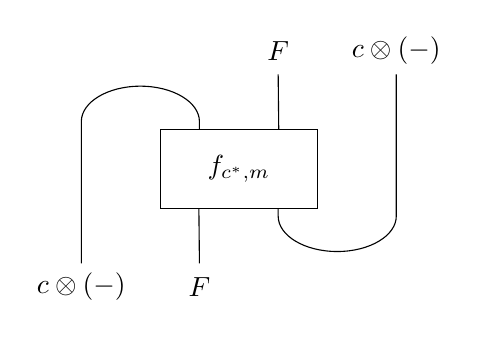
\begin{tikzpicture}[yscale=0.6]
	\node (A) at (2,2) [minimum height=1cm,minimum width=2cm, draw] {$f_{c^*,m}$};
	\draw (0,0) -- (0,3) arc (180:0:0.75cm) |- (A.135);
	\draw (A.225) -- (1.5,0);
	\draw (A.45) -- (2.5,4);
	\draw (A.315) -| (2.5,1) arc (180:360:0.75cm) -- (4,4);
	\node at (2.5,4.5) {$F$};
	\node at (4,4.5) {$c \otimes (-)$};
	\node at (0,-0.5) {$c \otimes (-)$};
	\node at (1.5, -0.5) {$F$};
\end{tikzpicture}
\end{center} 
We need to check that this map is inverse to $f_{c^*,m}$.  That this map is inverse to $f_{c^*,m}$ follows from the associativity condition for module functors and naturality, as illustrated here:
\begin{center}
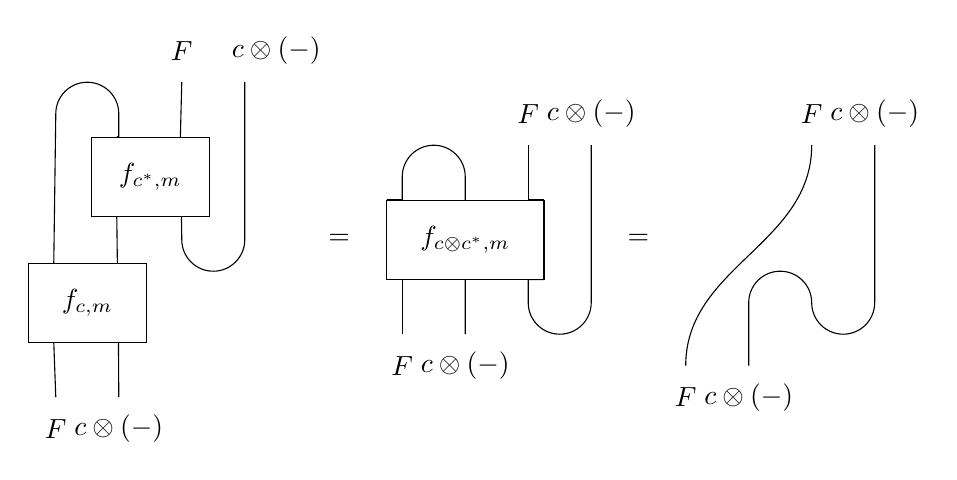
\begin{tikzpicture}[yscale=0.8, xscale=0.8, smooth]
	\node (A) at (2,2) [minimum height=1cm,minimum width=1.5cm, draw] {$f_{c^*,m}$};
	\node (B) at (1,0) [minimum height=1cm,minimum width=1.5cm, draw] {$f_{c,m}$};
	\draw (B.130) -- (.5,3) arc (180:0:0.5cm) |- (A.130) ;
	\draw (A.230) -- (B.53);
	\draw (A.53) -- (2.5,3.5);
	\draw (A.308) -- (2.5,1) arc (180:360:0.5cm) -- (3.5,3.5);
	\draw (B.308) -- (1.5, -1.5);
	\draw (B.230) -- (.5, -1.5);
	\node at (2.5,4) {$F$};
	\node at (4,4) {$c \otimes (-)$};
	\node at (.5, -2) {$F$};
	\node at (1.5, -2) {$c \otimes (-)$};
	
	\node at (5, 1) {$=$};
	
	\begin{scope}[xshift=5cm, yshift = -1cm]
		\node (A) at (2,2) [minimum height=1cm,minimum width=2cm, draw] {$f_{c \otimes c^*,m}$};
		\draw (A.153) -| (1,3) arc (180:0:0.5cm) -- (A.90) ;
		\draw (A.27) -| (3,3.5);
		\draw (A.333) -| (3,1) arc (180:360:0.5cm) -- (4, 3.5);
		\draw (A. 270) -- (2,.5);
		%\draw (A) -- (1,.5);
		\draw (A.207) -| (1,.5);
		\node at (3,4) {$F$};
		\node at (4,4) {$c \otimes (-)$};
		\node at (1,0) {$F$};
		\node at (2,0) {$c \otimes (-)$};
	\end{scope}
	
	\node at (9.75, 1) {$=$};
	
	\begin{scope}[xshift=10.5cm, yshift=-1cm]
		\draw (0, 0) to [out=90, in=270] (2,3.5);
		\draw (1,0) -- (1,1) arc (180:0:.5cm) arc (180:360:.5cm) -- (3,3.5);
		\node at (2,4) {$F$};
		\node at (3,4) {$c \otimes (-)$};
		\node at (0,-.5) {$F$};
		\node at (1,-.5) {$c \otimes (-)$};
	\end{scope}
\end{tikzpicture} \CD{straighten lines in the first picture?}  \NS{Done}
\end{center}
\end{proof}

The following Lemma was left as an exercise to the reader in \cite[\S 3.3]{EO-ftc}.

\begin{lemma} \label{lma:module-adjoint}
Let $\cC$ and $\cD$ be tensor categories. Let  $\cM$ and  $\cN$  be finite $\cC$--$\cD$-bimodule categories, and let $F: \cM \to \cN$ be a $\cC$--$\cD$-bimodule functor.  If the underlying functor of $F$ has a right (respectively left) adjoint as a functor, then $F$ has a right (respectively left) adjoint $\cC$--$\cD$-bimodule functor. \CD{notion of finite bimodule category hasn't specifically been introduced?}  \NS{Fixed, see note above}
\end{lemma}
\begin{proof}
Suppose that $G$ is the right adjoint to the underlying functor of $F$; we will show that $G$ naturally has the structure of a $\cC$--$\cD$-bimodule functor.  The result for left adjoints is similar.

The natural transformation $g_{c,n}: c \otimes G(n) \rightarrow G(c \otimes n)$ is given by the mate
$$c \otimes G(n) \rightarrow G F(c \otimes G(n)) \rightarrow G(c \otimes FG(n)) \rightarrow G(c \otimes n);$$
here the first map is the unit of the adjunction, the second map is the natural transformation given by the module functor structure on $F$, and the third map is the counit.  Diagrammatically: \CD{I removed all uses of `binatural'}
%\CSP{This looks wrong to me. It doesn't seem to match the formula. Maybe it rotates the same way as the previous one?}
%\NS{I think it's fixed now.  In some sense it rotates in the opposite direction as the previous argument, but we ended up doing the lax case for one and the oplax case for the other so they're the same.  Maybe that's misleading and we should change one of them.}
\begin{center}
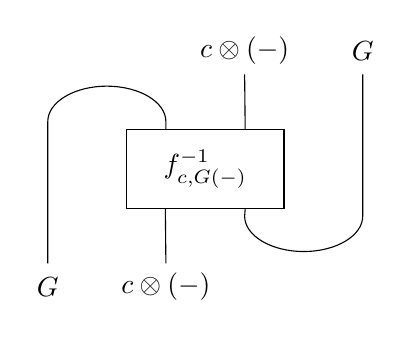
\begin{tikzpicture}[yscale=0.6]
	\node (A) at (2,2) [minimum height=1cm,minimum width=2cm, draw] {$f^{-1}_{c,G(-)}$};
	\draw (0,0) -- (0,3) arc (180:0:0.75cm) |- (A.135);
	\draw (A.225) -- (1.5,0);
	\draw (A.45) -- (2.5,4);
	\draw (A.315) -- (2.5,1) arc (180:360:0.75cm) -- (4,4);
	\node at (2.5,4.5) {$c \otimes (-)$};
	\node at (4,4.5) {$G$};
	\node at (0,-0.5) {$G$};
	\node at (1.5, -0.5) {$c \otimes (-)$};
\end{tikzpicture}
\end{center}

\noindent By the previous lemma, this natural transformation is an isomorphism.  Providing the structure of a $\cD$-module functor is similar, and these left and right module functor structures are compatible---that is they form a bimodule functor structure.
\end{proof}

\begin{remark}
If $\cC$ and $\cD$ are not rigid, the argument in the proof of this lemma only shows that the right adjoint to an oplax module functor has a lax module functor structure, while the left adjoint of a lax module functor has an oplax module functor structure.  %This is a serious issue as the following example shows. 
\end{remark}

\begin{lemma}\label{lem:partially_exact_action} \cite[Prop. 1.13.1]{EGNO} \cite[Prop. 2.1.8]{MR1797619}
	Let $\cC$ be a tensor category and let $\cM$ be a $\cC$-module category. Then for each object $c \in \cC$, the action map $c \otimes (-): \cM \to \cM$ is exact. 
\end{lemma}

\begin{proof}
	For each $c \in \cC$, the functor $c \otimes (-)$ admits both left and right adjoints, namely $c^* \otimes (-)$ and ${}^*c \otimes (-)$ respectively. 
\end{proof}



\subsection{Module categories are categories of modules}


Just as any finite linear category is a category of modules over an algebra, any finite module category over a finite tensor category is a category of module objects over an algebra object.  This result is one of the main theorems of \cite{EGNO}, and is essential to the structure theory of finite tensor categories.  The key construction underlying the proof is Ostrik's notion of the enriched hom for module categories \cite{MR1976459}.  

The following proposition is an elaboration of results of \cite{MR1976459} and \cite{EO-ftc}. % Really: enriched is due to EOFTC sec 3.2 (Ost03 did the semisimple case), the rest is new.
\begin{proposition} \label{thm:enrichment-of-mod-cats}
	Let $\cC$ be a finite linear monoidal category and let $\cM$ be a finite $\cC$-module category. Assume that the action map $\cC \times \cM \to \cM$ is right exact in each variable. 
		Then $\cM$ is enriched, tensored, and cotensored over $\cC$, with the tensor structure given by its structure as a $\cC$-module category. 
\end{proposition}

\begin{proof}
	We need functorial assignments of objects $\IHom(m', m) \in \cC$ and $m^c \in \cM$ for every $m,m' \in \cM$ and $c \in \cC$, and natural isomorphisms
	\begin{equation*}
		\Hom_\cC(c, \IHom(m', m)) \cong \Hom_\cM(c \otimes m', m) \cong \Hom_\cM( m', m^c)
	\end{equation*}
	witnessing adjunctions
	\begin{equation*}
			c \otimes - \quad \dashv\quad -^c \quad \textrm{ and } \quad - \otimes m' \quad \dashv \quad \IHom(m', -).
	\end{equation*}
Such assignments exist precisely if the functors
\begin{align*}
	\Hom_\cM(-\otimes m', m): \; & \cC^\op \to \Vect \\
	\Hom_\cM(c \otimes -, m): \; & \cM^\op \to \Vect
\end{align*}
are representable. The representing objects will be $\IHom(m', m)$ and $m^c$, respectively. Both of these functors are left exact, and hence by Corollary \ref{cor:representable} both of these functors are indeed representable.  %\NS{I fixed a broken reference here, hopefully I got the right one.}
\end{proof}

\begin{remark} \label{rem-enrich}
	The existence of the enrichment $\IHom(m', m)$ only requires $\cC$ to be finite and the action to be right exact in $\cC$, and similarly the existence of the cotensor $m^c$ only requires $\cM$ to be finite and the action to be right exact in $\cM$.
\end{remark}

\begin{example}
Consider $\Vect$ as a module category over $\Vect[K]$.  Then $\IHom(1,1)$ is $k[K]$ with each $g \in K$ having grading $g$.
\end{example}



The goal of this subsection is to prove a generalization of the following result. \CD{Need to explain specifically why we need a generalization of the result.}  \NS{We don't really need it, right?}

\begin{theorem}{\cite[Thm 2.11.6]{EGNO}, \cite[Thm 1]{MR1976459}} \label{thm:EGNO2.11.6}
	Let $\cM$ be a left module category over a finite tensor category $\cC$, and assume the action is right exact in $\cC$. If $\cM$ is finite as a linear category, then there exists an algebra object $A \in \cC$ together with an equivalence $\cM \simeq \Mod{}{A} (\cC)$ as left $\cC$-module categories. 
\end{theorem}

\begin{example} \label{eg:vect}
The $\Vect[K]$-module category $\Vect$ is equivalent to the category of modules over the algebra object $k[K] \in \Vect[K]$; here as before the element $g \in K$ has grading $g$.  
\end{example}

\begin{example} \label{ex:lax-module}
	In this theorem, it is necessary to assume $\cC$ is rigid.  Let $\cR \cong \Vect \oplus (\Vect \cdot X)$ be the non-rigid linear monoidal category consisting of pairs of vector spaces, which we write as $V_1 + V_2 X$, with tensor product given by 
	\begin{equation*}
		(V_1 + V_2 X) \otimes (W_1 + W_2 X) = V_1 \otimes W_1  +  (V_1 \otimes W_2 \oplus V_2 \otimes W_1)X.
	\end{equation*} 
	Up to equivalence there is a unique choice of associators and unitors making this a linear monoidal category. 
This is a categorification of the ring $k[x]/(x^2)$.  It is both finite and semisimple, but it is not rigid: the object $X$ cannot have a dual as there is no object $Z$ such that $Z \otimes X$ has a non-zero map to or from the unit object. 
	
	There is a tensor functor $F:\cR \to \Vect$ given by $(V_1 + V_2 X) \mapsto V_1$. This gives the category $\Vect$ the structure of a (left) $\cR$-module category, and moreover $F$ is naturally an $\cR$-module map. $F$ has both a left and a right adjoint, which agree and are given by the functor $G: \Vect \to \cR$ sending $W \in \Vect$ to $(W + 0 X) \in \cR$. \CD{say anything about reason for discussing adjoints of F?} \CD{why cf L2.10?} \NS{Should this say ``In contrast to L2.11"?}
	It is not possible to give $G$ the structure of a (strong) $\cR$-module functor (cf. Lemma~\ref{lem:laxisstrong}). Moreover there is no algebra object $A \in \cR$ such that $\Vect$ is equivalent to $\Mod{}{A}(\cR)$ as linear categories, let alone as $\cR$-module categories. \CD{last two sentences: clarify/spell out the logic/order of ideas here.}  \NS{I think we're just making claims, not proving them.  So there's no logic/order.}
\end{example}

In order to see how rigidity appears in the proof of the above theorem, we will first show a more general result that does not assume rigidity.

\begin{definition}
	Let $\cC$ be a finite linear monoidal category and let $\cM$ be a finite $\cC$-module category. Assume that the action is right exact in $\cC$, so $\cM$ is enriched over $\cC$ by Remark~\ref{rem-enrich}. 
	An object $p \in \cM$ will be called {\em $\cC$-projective} if $\IHom(p, -)$ is right exact (it is automatically left exact). An object $p$ will be called a {\em $\cC$-generator} if $\IHom(p,-)$ is faithful.
\end{definition}

\begin{remark} \label{rem:gen}
	An object $p \in \cM$ is a $\cC$-generator if and only if for each object $x \in \cM$ there exists an object $c \in \cC$ and a surjection $c \otimes p \twoheadrightarrow x$, which in turn is true if and only if for each object $x \in \cM$ the canonical map $\IHom(p,x) \otimes p \twoheadrightarrow x$ is a surjection. In particular an ordinary generator (i.e. an object such that $\Hom_\cM(p,-)$ is faithful) is also a $\cC$-generator.  \NS{Should this be a lemma instead of a remark?  I'm confused about the order in the first sentence and about why the last sentence follows.}
\end{remark}

\begin{example} \label{ex:rigid_all_C-proj}
	Let $\cC$ be a finite tensor category. We may view $\cC$ as a left $\cC$-module category over itself. Since $\cC$ is rigid, we have isomorphisms $\IHom(x,y) \cong y \otimes x^*$ and $(y^x) \cong {}^*x \otimes y$ (cf the proof of Lemma \ref{lma:RigidIsExact}). Moreover by Lemma \ref{lma:RigidIsExact}, in this case the tensor product is exact in each variable, hence every object of $\cC$ is $\cC$-projective, even those objects that are not projective in the usual sense. %\NS{To use that lemma you need to assume rigidity.}
\end{example}


\begin{theorem} \label{thm:C-module-Embedding} %!% [Thm 2.11.6(i)] 
	Let $\cM$ be a finite left module category over a finite (not necessarily rigid) linear monoidal category $\cC$. Assume that the action is right exact in $\cC$. 
	Fix an object $p \in \cM$, and set $A = \IHom(p,p) \in \cC$. The object $A$ is naturally an algebra object in $\cC$, and there is a $\cC$-module functor:
	\begin{align*}
		F:   \Mod{}{A}(\cC) \to \cM \\
		F(x_A) := \coeq \left( x \otimes \IHom(p,p) \otimes p \rightrightarrows x \otimes p \right).
	\end{align*}
The functor $\IHom(p,-): \cM \to \Mod{}{A}(\cC)$ is right adjoint to $F$. 

Assume that $\IHom(p,-)$ may be equipped with the structure of a $\cC$-module functor and that the unit and counit of the adjunction $F \dashv \IHom(p,-)$ are morphisms of $\cC$-module functors. Assume further that $p$ is a $\cC$-projective $\cC$-generator.  Then the $\cC$-module adjunction  $F \dashv \IHom(p,-)$
	induces an equivalence of left $\cC$-module categories $\cM \simeq \Mod{}{A}(\cC)$. 
\end{theorem}

\noindent The proofs given in \cite{EGNO} and \cite{MR1976459} at first appear to depend on  the rigidity of $\cC$. Indeed the first step of the proof of \cite[Thm 2.11.2]{EGNO} invokes \cite[lemma 2.10.4.(4)]{EGNO} whose proof makes explicit use of rigidity. The same lemma is used in step (3) of the proof of \cite[Thm 1]{MR1976459}. However with a little care the rigidity assumption can be avoided (cf. \cite[Rmk. 2.11.3]{EGNO}).  

\begin{proof}[Proof of Thm.~\ref{thm:C-module-Embedding}]
	We have a series of natural isomorphisms:
	\begin{align*}
		\Hom_{\Mod{}{A}(\cC)}&(b, \IHom(p,x))  \cong \Hom_{\Mod{}{A}(\cC)}( \coeq \left( b \otimes A \otimes A_A \rightrightarrows b \otimes A_A  \right), \IHom(p,x)) \\
		& \cong \eq \left( \Hom_{\Mod{}{A}(\cC)}(b \otimes A_A, \IHom(p,x) )  \rightrightarrows \Hom_{\Mod{}{A}(\cC)}(  b \otimes A \otimes A_A, \IHom(p,x))  \right) \\
		& \cong \eq \left( \Hom_{\cC}(b, \IHom(p,x) )  \rightrightarrows \Hom_{\cC}(  b \otimes A, \IHom(p,x))  \right) \\
		& \cong \eq \left( \Hom_{\cM}(b \cdot p, x )  \rightrightarrows \Hom_{\cM}(  (b \otimes A) \cdot p, x)  \right) \\
		& \cong  \Hom_{\cM}( \coeq \left( (b \otimes \IHom(p,p)) \cdot p \rightrightarrows b \cdot p \right), x) \\
		& \cong \Hom_{\cM}( F(b), x)
	\end{align*}  \CD{explain use of dot notation? just use otimes?} \NS{The cong's were missing on the last two lines, so I added them}
	where $b \in \Mod{}{A}(\cC)$ and $x \in \cM$. This establishes that $\IHom(p,-): \cM \to \Mod{}{A}(\cC)$ is indeed right adjoint to $F$.

For the second part of the theorem, our assumptions ensure that:
\begin{enumerate}
	\item the functor $\IHom(p, -)$ commutes (coherently) with the $\cC$-action; \CD{omit item (1)}
	\item the functor $\IHom(p, -)$ is fully-faithful; and \CD{say anything about full?}
	\item the functor $\IHom(p, -)$ is exact; 
\end{enumerate}
We wish to show that $\IHom(p, -)$ induces an equivalence of $\cC$-module categories. By Lemma \ref{lem:Recog_equiv_of_bimod} and (1), it is enough to show that it induces an equivalence of underlying categories. Moreover by (2) it is enough to show that the unit map $B \to \IHom(p, F(B))$ is an equivalence for all right $A$-modules $B$. This last statement holds by the following sequence of isomorphisms (which use (2) and (3) and the $\cC$-module structure on $\IHom$):
\begin{align*}
	B & \cong \coeq \left( B \otimes \IHom(p,p) \otimes \IHom(p,p) \rightrightarrows B \otimes \IHom(p,p) \right)\\
	& \cong \coeq \left(\IHom(p,B  \otimes \IHom(p,p) \otimes p) \rightrightarrows \IHom(p,B \otimes p) \right)\\
	& \cong \IHom(p, F(B)). \qedhere
\end{align*}	
\end{proof}

%The Barr-Beck monadicity theorem\NS{Citation for Barr-Beck} implies that $\cM$ is equivalent to the category of algebras in $\cC$ for the monad $\IHom(p, (-) \otimes p)$. If the adjunction is $\cC$-linear, so in particular $\IHom(p,-)$ is a $\cC$-module functor, then this monad will be a ``$\cC$-module monad''. In this case the category of algebras for this monad is a $\cC$-module category and is easily identified with $\Mod{}{A}(\cC)$. \NS{Should this be written as an actual proof?}

If we additionally assume that $\cC$ is rigid, then some of the conditions of the previous theorem are automatically satisfied and become redundant. In particular Lemma \ref{lma:module-adjoint} implies that when $\cC$ is rigid the functor $\IHom(p,-)$ can always be enhanced to a $\cC$-module functor.  The following lemma shows that in this case there always exists a $\cC$-projective $\cC$-generator.  
\begin{lemma}{\cite[\S 2.11]{EGNO}} \label{lma:Enough_C-projs}
	If $\cC$ is a finite tensor category and $\cM$ is a finite module category in which the action is right exact in $\cC$, then there exists a $\cC$-projective $\cC$-generator. \CD{Has `finite module category' been used before?}  \NS{Fixed above}
\end{lemma}   
\begin{proof}
	We claim that if $p \in \cM$ is a projective object (in the ordinary sense) then it is also $\cC$-projective. If this claim holds, then any (ordinary) projective generator of $\cM$ will be a $\cC$-projective $\cC$-generator (cf Remark \ref{rem:gen}), and projective generators are guaranteed to exist since $\cM$ is finite. \CD{say anything about existence of generator?}
	Thus assume that $p \in \cM$ is projective.  We need to show that $\IHom(p, -)$ is right exact. 
	
	Since $\cC$ is rigid, we have a natural isomorphism of functors:
\begin{equation*}
	\Hom_{\cM}(c \otimes p, m) \cong \Hom_{\cM}(p, {}^*c \otimes m).
\end{equation*}
Taking an object to its dual is a (contravariant) equivalence of categories hence is exact. Moreover since $p$ is projective and the $\cC$-module structure is right exact, we see that the functor $\Hom_{\cM}(- \otimes p, -)$ is left exact in the first variable and right exact in the second variable. Said another way, for each projective $p \in \cM$ we have a right exact functor
\begin{align*}
	G_p: & \; \cM \to \Fun^L(\cC^\op, \Vect) \\
	& m \mapsto (c \mapsto \Hom_{\cM}(c \otimes p, m)).
\end{align*} \CD{L/R given op ...}
By Proposition \ref{thm:enrichment-of-mod-cats} this functor factors through the Yoneda embedding as
\begin{equation*}
	\IHom(p, -): \cM \to \cC.
\end{equation*}
Thus if $m \to m' \to m'' \to 0$ is an exact sequence in $\cM$ and $x \in \cC$ is any object we have an exact sequence
\begin{equation*}
	\Hom(x, \IHom(p,m)) \to \Hom(x, \IHom(p,m')) \to \Hom(x, \IHom(p,m'')) \to 0.
\end{equation*}
In particular this holds when $x$ is a projective generator (which is guaranteed to exist since $\cC$ is finite). It follows that 
\begin{equation*}
	\IHom(p,m) \to \IHom(p,m') \to \IHom(p,m'') \to 0
\end{equation*}
is an exact sequence: if $x \in \cC$ is a projective generator, then a sequence $y \to y' \to y'' \to 0$ in $\cC$ is exact if and only if 
\begin{equation*}
	\Hom(x, y) \to \Hom(x, y') \to \Hom(x, y'') \to 0
\end{equation*} 
is exact. 
\end{proof}




\begin{proof}[Proof of Thm.~\ref{thm:EGNO2.11.6}]
By Lemmas \ref{lma:Enough_C-projs} and \ref{lma:module-adjoint}, the assumptions of Theorem~\ref{thm:C-module-Embedding} are satisfied.
\end{proof}

\begin{corollary} \label{cor:biexact_action}
	Let $\cC$ be a finite tensor category and let $\cM$ be a finite $\cC$-module category. If the action map $\cC \times \cM \to \cM$ is right exact in $\cC$, then the action is in fact exact in each variable separately.  
\end{corollary}

\begin{proof}
	By Lemma~\ref{lem:partially_exact_action} the functor $c \otimes (-)$ is exact for each $c \in \cC$. We must show that $(-) \otimes m$ is exact for each $m \in \cM$. By Theorem~\ref{thm:EGNO2.11.6} there exists an algebra object $A \in \cC$, and an equivalence of $\cC$-module categories $\cM \simeq \Mod{}{A}(\cC)$. Hence there exists a forgetful functor $U:\cM \to \cC$ which is a $\cC$-module functor, is exact, and reflects short exact sequences. It follows that $(-) \otimes m: \cC \to \cM$ is exact if and only if $(-) \otimes U(m): \cC \to \cC$ is exact, but this follows from Lemma~\ref{lma:RigidIsExact}. 
\end{proof}

\begin{remark}
	By taking opposite categories, in the above corollary one may replace `right exact in $\cC$' with `left exact in $\cC$'. 
\end{remark}


\section{Construction of the balanced tensor product} \label{sec:tc-deligne}

In this section establish the existence of the balanced tensor product of finite module categories over a finite tensor category.  We begin by recalling the definition of the balanced tensor product from \cite{0909.3140}.


\begin{definition}
	Let $\cC$ be a linear monoidal category. 
	Let $\cM$ be a right $\cC$-module category and $\cN$ a left $\cC$-module category. A {\em $\cC$-balanced functor} into a linear category $\cL$ is a right exact bilinear functor $F: \cM \times \cN \to \cL$ together with a natural isomorphism $F(\otimes^{\cM} \times \id_{\cN}) \cong F(\id_{\cM} \times \otimes^{\cN})$ satisfying the evident pentagon identity. \CD{Did we say what right exact bilinear means?}
	A {\em $\cC$-balanced transformation} is a natural transformation $\eta:F \to G$ of $\cC$-balanced functors such that the following diagram commutes for all $m \in \cM$, $c \in \cC$, and $n \in \cN$:
\begin{center}
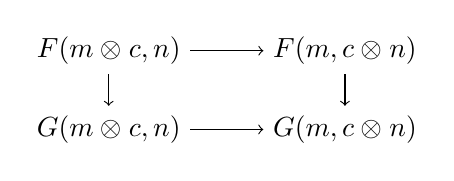
\begin{tikzpicture}
	\node (LT) at (0, 1) {$F(m \otimes^{\cM} c, n)$};
	\node (LB) at (0, 0) {$G(m \otimes^{\cM} c, n)$};
	\node (RT) at (3, 1) {$F(m, c \otimes^{\cN} n)$};
	\node (RB) at (3, 0) {$G(m, c \otimes^{\cN} n)$};
	\draw [->] (LT) -- node [left] {$$} (LB);
	\draw [->] (LT) -- node [above] {$$} (RT);
	\draw [->] (RT) -- node [right] {$$} (RB);
	\draw [->] (LB) -- node [below] {$$} (RB);
	%\node at (0.5, 1) {$\ulcorner$};
	%\node at (1.5, 0.5) {$\lrcorner$};
\end{tikzpicture}.
\end{center}
\end{definition}


\begin{definition}
	Let $\cM$ be a right $\cC$-module category and let $\cN$ be a left $\cC$-module category. The {\em balanced tensor product} is a linear category $\cM \boxtimes_{\cC} \cN$
	 together with a $\cC$-balanced right exact bilinear functor $\boxtimes_{\cC} : \cM \times \cN \to \cM \boxtimes_{\cC} \cN$, such that for all linear categories $\cD$, the functor $\boxtimes_{\cC}$ induces an equivalence between the category of $\cC$-balanced right exact bilinear functors $\cM \times \cN \to \cD$ and the category of right exact linear functors $\cM \boxtimes_{\cC} \cN \to \cD$. \CD{changed this def}
\end{definition}
\nid More succinctly, we might say, the balanced tensor product $\cM \boxtimes_{\cC} \cN$ corepresents $\cC$-balanced right exact bilinear functors out of $\cM \times \cN$.  The balanced tensor product is also known as the ``relative Deligne tensor product", because the (unbalanced) tensor product $\cM \boxtimes \cN$ of linear categories is often called the ``Deligne tensor product".  

If it exists, the balanced tensor product is unique up to equivalence, and this equivalence is in turn unique up to unique natural isomorphism. Said another way, the 2-category of linear categories representing the balanced tensor product is either contractible or empty. 

Etignof--Nikshych--Ostrik \cite{0909.3140} established the existence of the balanced tensor product of semisimple module categories over semisimple tensor categories over a field of characteristic zero.  A construction of the balanced tensor product for finite tensor categories satisfying the additional assumption that $\cM \boxtimes \cN$ is exact as a $\cC$-bimodule category can be extracted from \cite[Thm 3.1]{1102.3411}. \CD{rephrase and deal with the fact that exact hasn't been mentioned}  \NS{I think it's fine as is.  People don't need to know what exactness means for this paper, and if they want to know they can read the referenced paper.}
 The following theorem extends these results to arbitrary finite tensor categories and finite module categories. 

\begin{theorem} \label{thm:DelignePrdtOverATCExists}
	Let $\cC$ be a finite tensor category and let $\cM_{\cC}$ and ${}_{\cC}\cN$ be finite right and left $\cC$-module categories, respectively. Assume that the action of $\cC$ on $\cM$ and the action of $\cC$ on $\cN$ are right exact in the $\cC$-variable.
	\begin{enumerate}
		\item The balanced tensor product $\cM \boxtimes_{\cC} \cN$ exists and is a finite linear category.
		\item If $\cM = \Mod{A}{}(\cC)$ and $\cN = \Mod{}{B}(\cC)$, then $\cM \boxtimes_{\cC} \cN \simeq \Mod{A }{B}(\cC)$, the category of $A$--$B$-bimodule objects in $\cC$.

		\item The functor $\boxtimes_{\cC}: \cM \times \cN \to \cM \boxtimes_{\cC} \cN$ is exact in each variable and satisfies 
		\begin{equation*}
			\Hom_{\cM}(x,x') \otimes \Hom_{\cN}(y, y') \cong \Hom_{\cM \boxtimes_{\cC} \cN} (x \boxtimes_{\cC} y, x' \boxtimes_{\cC} y').
		\end{equation*}
		\item Given exact $\cC$-module functors $F_0: M \to M'$ and $F_1: N \to N'$, the $\cC$-balanced functor $F: M \times N \to M' \times N' \to M' \boxtimes_{\cC} N'$ induces an exact functor $\overline{F}: M \boxtimes_{\cC} N \to M' \boxtimes_{\cC} N'$.
	\end{enumerate} 
\end{theorem}


\begin{proof}
	 By Theorem \ref{thm:EGNO2.11.6}, there exist algebra objects $A, B \in \cC$ and equivalences $\cM \simeq \Mod{A}{}(\cC)$ and $\cN \simeq \Mod{}{B}(\cC)$. By Lemma \ref{lma:RigidIsExact}, the tensor product functor
	\begin{equation*}
		\cM \times \cN \simeq \Mod{A}{}(\cC) \times  \Mod{}{B}(\cC) \to \Mod{A}{B}(\cC)
	\end{equation*}
	is exact in each variable separately. It is also $\cC$-balanced by the associator of $\cC$.\NS{I added what the balancing is.} Thus $(2)$ implies both  $(1)$ and $(3)$. \CD{(1) discuss why A-Mod-B(C) is finite. (3) discuss displayed relation.}
	We will first prove (2), and then establish (4).  We wish to show that for any $\cD$ the category of right exact functors 
\begin{equation*}
	\overline{F}:\Mod{A}{B}(\cC) \to \cD
\end{equation*}
	is naturally equivalent to the category of $\cC$-balanced functors $F:\cM \times \cN \to \cD$ that are right exact in each variable separately. Every functor of the former type certainly restricts to one of the later type; we must show that a functor of the latter type extends uniquely (up to canonical isomorphism) to one of the former type. \CD{`uniquely (up to canon iso)' is not an entirely accurate description of what's required, right? (we just need any inverse, which will happen to be unique because inverses are unique ...)}
	
The key observation is that every object of $\Mod{A}{B}(\cC)$ may be functorially written as a coequalizer of objects in the image of $\cM \times \cN$. Specifically, for any $X \in \Mod{A}{B}(\cC)$, we have the coequalizer:
\begin{equation*}
	{}_A A \otimes A \otimes X_B \rightrightarrows {}_A A \otimes X_B \to {}_A X_B.
\end{equation*}
Let $\delta: {}_A A \otimes A \otimes X_B \to {}_A A \otimes X_B$ be the difference of the two maps in the coequalizer. 
For any right exact functor $\overline{F}: \Mod{A}{B}(\cC) \to \cD$, the value $\overline{F}({}_A X_B)$ is canonically determined as a cokernel:
\begin{equation*}
	\overline{F}({}_A X_B) = \coker \left( \overline{F}(\delta): \overline{F}({}_A A \otimes A \otimes X_B) \to \overline{F}({}_A A \otimes X_B) \right).
\end{equation*} 
	
Suppose we are given a $\cC$-balanced functor $F:\cM \times \cN \to \cD$ that is right exact in each variable separately. It is tempting to try to define the extension $\overline{F}: \Mod{A}{B}(\cC) \to \cD$ via a formula of the type:
\begin{equation*}
	``\overline{F}({}_A X_B) := \coker \left( F(\delta): F({}_A A \otimes A,  X_B) \to {F}({}_A A , X_B) \right)."
\end{equation*} 
The difficulty is that while the relevant objects are in the image of $\cM \times \cN$, the map $\delta$ is not. 
Yet for each $X \in \Mod{A}{B}(\cC)$ we may form the following commutative diagram. 
%shown in Figure %\ref{fig:RelDelingePdtDiagram}.
%\begin{figure}[htbp]
	\begin{center}
		\begin{tikzpicture} \matrix (m) [matrix of math nodes, row sep={1.5cm,between origins}] {
		 F({}_AA \otimes A \otimes X, B \otimes B_B) &[1cm] F({}_AA \otimes X, B \otimes B_B) &[1cm] F({}_A X, B \otimes B_B) &[0.5cm] 0 \\
		F({}_AA \otimes A, X \otimes B \otimes B_B) & F({}_AA, X \otimes B \otimes B_B) & & \\
		F({}_AA \otimes A, X \otimes B_B) & F({}_AA , X \otimes B_B) & & \\
		 F({}_AA \otimes A \otimes X, B_B) & F({}_AA \otimes X, B_B) & F({}_AX,B_B)  & 0 \\
		& &\coker(\overline{\delta}_X)  & \\
			};
			\draw [->] (m-1-1) -- node [above] {$\delta_1$} (m-1-2);
			\draw [->] (m-1-2) -- node [above] {$$} (m-1-3);
			\draw [->] (m-1-3) -- node [above] {$$} (m-1-4);
			\draw [->] (m-4-1) -- node [above] {$\delta_1$} (m-4-2);
			\draw [->] (m-4-2) -- node [above] {$$} (m-4-3);
			\draw [->] (m-4-3) -- node [above] {$$} (m-4-4);
			\draw [->] (m-1-1) -- node [left] {$\cong$} (m-2-1);
			\draw [->] (m-1-2) -- node [left] {$\cong$} (m-2-2);
			\draw [->] (m-3-1) -- node [left] {$\cong$} (m-4-1);
			\draw [->] (m-3-2) -- node [left] {$\cong$} (m-4-2);
			\draw [->] (m-2-1) -- node [left] {$\delta_2$} (m-3-1);
			\draw [->] (m-2-2) -- node [left] {$\delta_2$} (m-3-2);
			\draw [->,dashed] (m-1-3) -- node [left] {$\overline{\delta}_X$} (m-4-3);
			\draw [->,dashed] (m-4-3) -- node [left] {$$} (m-5-3);
			\node [node distance = 1.75cm, right of= m-5-3] {$=:\overline{F}({}_AX_B)$};
		\end{tikzpicture}
	\end{center}
%	\caption{A digram useful for demonstrating the existence of the balanced tensor product.}
%	\label{fig:RelDelingePdtDiagram}
%\end{figure}
\CD{Why was the tempting map on the other side from the construction?}
Here the arrows labeled with isomorphisms come from the $\cC$-balanced structure of the functor $F$, while the remaining solid arrows are maps in the image of $\cM \times \cN$. The maps labeled with either $\delta_1$ or $\delta_2$ represent difference maps of maps in $\cM$ or $\cN$, as above.  (The fact that this diagram commutes uses the coherence and naturality of the $\cC$-balanced structure. To verify the commutativity it is easiest to break each difference map into its constituent piece (one from the multiplication in either $A$ or $B$, and one from the action on $X$) and to show commutativity with respect to these maps.)

The rows of this diagram are exact (since $F$ was assumed to be right exact in each variable) and hence this diagram defines a unique map $\overline{\delta}_X$, shown as the long dashed arrow. We may define the value of the extension $\overline{F}$ on the object ${}_AX_B$ as the cokernel of $\overline{\delta}_X$. We leave it to the reader to verify that this extension gives a well-defined right exact functor 
\begin{equation*}
	\overline{F}: \Mod{A}{B}(\cC) \to \cD,
\end{equation*} 
and implements the desired equivalence between such right exact functors and $\cC$-balanced exact-in-each-variable functors. Verifying that this construction is well defined makes use of the pentagon identity satisfied by $\cC$-balanced functors. This establishes (1), (2), and (3). 

We now prove the final property (4). By Theorem \ref{thm:EGNO2.11.6}, there exist algebra objects $A, B, A'$, and $B' \in \cC$ and equivalences $\cM \simeq \Mod{A}{}(\cC)$, $\cN \simeq \Mod{}{B}(\cC)$, $\cM' \simeq \Mod{A'}{}(\cC)$, and $\cN \simeq \Mod{}{B'}(\cC)$. Since $F_0$ and $F_1$ are right exact, they are equivalent to tensoring with bimodules:
\begin{align*}
	F_0(-) &\cong {}_{A'}x \otimes_A (-); \\
	F_1(-) & \cong (-) \otimes_B y_{B'}.
\end{align*}
Since $F_0$ and $F_1$ are exact, we may call these modules {\em flat} over $A$ or $B$, respectively. We wish to show that the induced functor:
\begin{equation*}
	\overline{F}(-) = {}_{A'}x \otimes_A (-) \otimes_B y_{B'}: \Mod{A}{B}(\cC) \to \Mod{A'}{B'}(\cC)
\end{equation*}
is exact. Since the forgetful functor $U: \Mod{A'}{B'}(\cC) \to \cC$ is exact and reflects short exact sequences, it is enough to show that 
\begin{equation*}
	x \otimes_A (-) \otimes_B y: \Mod{A}{B}(\cC) \to \cC
\end{equation*}
is exact. Let $0 \to m \to m' \to m'' \to 0$ be a short exact sequence of $A$--$B$-bimodules. After tensoring with $x$ on the left we obtain a sequence of right $B$-modules:
\begin{equation*}
	0 \to x \otimes_A m \to x \otimes_A m' \to x \otimes_A {m''} \to 0
\end{equation*}
Since $x$ is flat, this sequence is exact after forgetting the $B$-module structure. Hence it is also an exact sequence of $B$-modules. Thus, since $y$ is flat, we obtain an exact sequence
\begin{equation*}
		0 \to x \otimes_A m \otimes_B y \to x \otimes_A m'\otimes_B y \to x \otimes_A {m''}  \otimes_B y \to 0
\end{equation*}
	as desired. 
%The final property, part (4), now follows from a routine diagram chase, which we also leave to the reader. 
\end{proof}

\begin{example}
The balanced product $\Vect \boxtimes_{\Vect[K]} \Vect$ is the category of $k[K]$-bimodules in $\Vect[K]$. As mentioned in Example~\ref{eg:vect}, the category of $k[K]$-modules in $\Vect[K]$ is equivalent to $\Vect$, so the $k[K]$-bimodules in $\Vect[K]$ can be identified with $\text{mod-}k[K] \cong \Rep(K)$.
\end{example}

\begin{remark}
	If ${}_{\cD}\cM_{\cC}$ and ${}_{\cC}\cN_{\cE}$ are bimodule categories, then the actions of $\cD$ and $\cE$ induce a $\cD$--$\cE$-bimodule category structure on $\cM \boxtimes_{\cC} \cN$. This bimodule category satisfies the analogous universal property for $\cC$-balanced bilinear bimodule functors.
\end{remark}

\begin{remark}
The above theorem assumes that $\cC$ is a finite tensor category, that is a finite rigid linear monoidal category.  The non-balanced tensor product can be defined substantially more generally \cite{1212.1545}, and we hope that the balanced tensor product can also be defined more generally.
\end{remark}
\CD{Add comment on importance/essentialness of right exactness in the theorem?}

\subsection{Properties of the unbalanced tensor product}
\CD{The rest seems weirdly tacked on.  Feels like the paper ends here properly.  Not sure what to do about that.}  \NS{We need these results, and I think this paper is a more appropriate place for it than DTC.  They have to go after the main results.  I wouldn't object to it being made an appendix.  But as usual I don't care whether a paper ends on a high note, people rarely read to the end of papers anyway.}

In the case where $\cC = \Vect$, and we are working over a perfect field, the exactness descent property given in Part (4) of Theorem~\ref{thm:DelignePrdtOverATCExists} can be strengthened as follows.

\begin{lemma}[{\cite[Pr.~5.13(vi)]{MR1106898}}]%\label{lem:}
	Suppose that $\cM$, $\cN$, and $\cP$ are finite linear categories and the functor $F: \cM \times \cN \to \cP$ is exact in each variable separately. If the ground field is perfect, then the induced functor $\overline{F}: \cM \boxtimes \cN \to \cP$ is exact. 
\end{lemma} \CD{rephrased this}

This has a crucial consequence. The Deligne tensor product of finite tensor categories will always be a finite monoidal linear category, but over a perfect field we have:

\begin{corollary}[{\cite[Pr.~5.17]{MR1106898}}]%\label{cor:}
	If the ground field is perfect, then tensor product of finite tensor categories is rigid, and hence again a tensor category. 
\end{corollary}

\begin{example}
	The assumption that the ground field is perfect is essential. If $k$ is imperfect, let $L$ be a finite inseparable field extension. The category $\Vect_L$ of $L$-vector spaces, with the usual tensor product over $L$, is a semisimple tensor category. However the Deligne tensor product $\Vect_L \boxtimes_{\Vect_k} \Vect_L$
	is equivalent to the category of $L \otimes L$-modules. This category is no longer semisimple (since $L$ is inseparable) and moreover the induced monoidal structure is the tensor product over $L \otimes L$, which is no longer exact in each variable. It follows (cf. Lemma~\ref{lma:RigidIsExact}) that $\Vect_L \boxtimes_{\Vect_k} \Vect_L$ fails to be rigid. 
\end{example} \CD{Spell this example out more (also phrase in a way that makes it clear semisimplicity comments are unrelated to rigidity comments?)}

Finally we observe that the product of two internal module categories is an internal module category over the product algebra object:

\begin{proposition}
	%\label{lem:}
	If $\cN = \Mod{}{B}(\cC)$ and $\cP = \Mod{}{C}(\cD)$, for algebra objects $B \in \cC$ and $C \in \cD$, then $$\cN \boxtimes \cP \simeq \Mod{}{(B \boxtimes C)}(\cC \boxtimes \cD)$$ as a left $\cC \boxtimes \cD$-module category.
\end{proposition}

\begin{proof}
	The forgetful functors from $\cN$ to $\cC$ and $\cP$ to $\cD$ are part of monadic adjunctions:
	\begin{align*}
		(-) \otimes B_{B}:\cC \rightleftarrows \cN = \Mod{}{B}(\cC): U \\
		(-) \otimes C_{C}:\cD \rightleftarrows \cP = \Mod{}{C}(\cD): U
	\end{align*}
	Since both functors in the adjunction are right exact (the forgetful functor is exact, not just left exact) these adjunctions descend to an adunction between the tensor products. 
	\begin{equation*}
		(-) \otimes (B \boxtimes C)_{B \boxtimes C}: \cC \boxtimes \cD \rightleftarrows \cN \boxtimes \cP: \overline{U}.
	\end{equation*}
	Any $\cC \boxtimes \cD$-module functor from $\cC \boxtimes \cD$ to itself is given by tensoring by an object in $\cC \boxtimes \cD$, hence any monad on $\cC \boxtimes \cD$ that is compatible with the module actions comes from an algebra in $\cC \boxtimes \cD$.  \CD{Isn't this sentence irrelevant? omit.}
	Hence we need only show that this adjunction is monadic.  
	
	\NS{I added stuff here about why the theorem follows from monadicity of the adjunction, since it was not obvious to me until I spent a while thinking about it.}
	
	By the the crude monadicity theorem \cite[\S~3.5]{MR771116} we only need to show that $\overline{U}$ reflects isomorphisms and $\overline{U}$ preserves coequalizers of reflexive pairs.  The former follows from the five lemma and the fact that everything in $\cC \boxtimes \cD $ is a coequalizer of objects in the image of $\cN \times \cP$.  \CD{Explain fact more.} \CD{Explain follows more?}
	For the latter we show that $\overline{U}$ preserves all coequalizers. Since our categories are additive the coequalizer of $f$ and $g$ is the cokernel of $(f-g)$.  Thus it is sufficient to show that $\overline{U}$ is exact and hence that $\overline{U}$ preserves cokernels.  The exactness of $\overline{U}$ follows from Part (4) of Theorem~\ref{thm:DelignePrdtOverATCExists} and exactness of the original forgetful functors $U$.  
\end{proof}

\CD{Switch order of DSPS13a and DSPS13b in the biblio, cf lurie entries for how}

\bibliographystyle{alpha}
\bibliography{dtcbib}
\end{document}
